\documentclass{article}

%\renewcommand{\baselinestretch}{1.5}
\usepackage{mathtools}
\usepackage[utf8]{inputenc}
\usepackage{amsmath}
\usepackage{amssymb}
\usepackage{graphicx}
\usepackage{bm}
\usepackage{enumitem}
\usepackage{textcomp}
\DeclarePairedDelimiter\ceil{\lceil}{\rceil}
\DeclarePairedDelimiter\floor{\lfloor}{\rfloor}

\usepackage[margin=1in]{geometry}

\setlength\parindent{0pt}
%\setlength{\parskip}{5px}
\setlength{\parskip}{1em}

\newtheorem{lemma}{Lemma}

\newcommand\at[2]{\left.#1\right|_{#2}}
\newcommand{\p}[2]{\frac{\partial #1}{\partial #2}}
\newcommand{\abs}[1]{\left| #1 \right|}
\newcommand{\paren}[1]{\left(#1\right)}
\newcommand{\brac}[1]{\left[#1\right]}
\newcommand{\R}{\mathbb{R}}
\newcommand{\Z}{\mathbb{Z}}
\newcommand{\C}{\mathbb{C}}

\DeclareMathOperator{\var}{var}
\DeclareMathOperator{\real}{Re}
\DeclareMathOperator{\imm}{Im}
\DeclareMathOperator{\Arg}{Arg}
\DeclareMathOperator{\Log}{Log}
\DeclareMathOperator{\Res}{Res}

\title{MA3111 AY1819 Sem 2 Solutions}
\author{Lim Li}

\begin{document}
\maketitle
\begin{enumerate}
\item
\[(2i)^{5/4} = 2^{5/4}(e^{i\frac{\pi}{2}})^{5/4} = 2^{5/4} (e^{i\frac{\pi}{2}})^{1/4} = 2^{5/4} e^{i(\frac{\pi}{8} + \frac{\pi n}{2})}, \quad n=0,1,2,3\]
\begin{align*}
\Log ((2i)^{5/4}) &= \Log(2^{5/4} e^{i(\frac{\pi}{8} + \frac{\pi n}{2})}) \\
    &= \ln(2^{5/4}) + i\Arg(e^{i(\frac{\pi}{8} + \frac{\pi n}{2})}) \\
    &= \frac{5}{4} \ln 2 + i\Arg(e^{i(\frac{\pi}{8} + \frac{\pi n}{2})})
\end{align*}
It could take on values $\frac{5}{4} \ln 2 + i\Arg(e^{i(\frac{\pi}{8} + \frac{\pi n}{2})})$ for $n=0,1,2,3$.

$(\frac{5}{4} \ln 2 , \frac{\pi}{8})$, $(\frac{5}{4} \ln 2 , \frac{5\pi}{8})$, $(\frac{5}{4} \ln 2 , -\frac{7\pi}{8})$, $(\frac{5}{4} \ln 2 , -\frac{3\pi}{8})$
\item
\begin{enumerate}
\item Note that
\[\frac{1}{z+c} = \frac{1}{c} - \frac{z}{c^2} + \frac{z^2}{c^3} - \cdots\]
Hence,
\begin{align*}
\frac{z^3-1}{z^2+3z-4} &= (z^2+z+1)\paren{\frac{1}{z+4}} \\
    &= (z^2+z+1)\paren{\frac{1}{4} - \frac{z}{4^2} + \frac{z^2}{4^3} - \cdots} \\
    &= \frac{1}{4} + (\frac{1}{4} - \frac{1}{16})z + (\frac{1}{4} - \frac{1}{4^2} + \frac{1}{4^3})z^2 + \cdots \\
    &= \frac{1}{4} + \frac{3}{16} z + \frac{13}{64} z^2 + \cdots
\end{align*}
The first 3 terms of the taylor series is $\frac{1}{4}, \frac{3}{16}, \frac{13}{64}$.

Note that the radius of convergence of $\frac{1}{z+4}$ is 4, and $(z^2 + z + 1)$ converges everywhere. Hence, the radius of convergence of $\frac{z^3-1}{z^2+3z-4} = (z^2 + z + 1)\paren{\frac{1}{z+4}}$ is 4.
\item
\[
\frac{1}{z+4} = \frac{1}{3} - \frac{z+1}{3^2} + \frac{(z+1)^2}{3^3} - \cdots
\]
\begin{align*}
\frac{z^3-1}{z^2+3z-4} &= ((z+1)^2 - (z+1) + 1)\paren{\frac{1}{z+4}} \\
    &= ((z+1)^2 - (z+1) + 1)\paren{\frac{1}{3} - \frac{z+1}{3^2} + \frac{(z+1)^2}{3^3} - \cdots} \\
    &= \frac{1}{3} + \paren{-\frac{1}{3^2} - \frac{1}{3}}(z+1) + \paren{\frac{1}{3^3} + \frac{1}{3^2} + \frac{1}{3}}(z+1)^2 + \cdots
\end{align*}
Hence,
\[
\frac{z^3-1}{z^2+3z-4} = \sum_{n=0}^\infty a_n (z+1)^n
\]
where
\[a_0 = \frac{1}{3}\]
\[a_1 = -\frac{4}{9}\]
\[
a_n = (-1)^n\paren{\frac{1}{3^{n+1}} + \frac{1}{3^{n}} + \frac{1}{3^{n-1}}}, \quad \text{for }n\geq 2
\]
\end{enumerate}
\item
\begin{enumerate}
\item $f(z)$ is not analytic when $z=0$ and when $\sin(\pi z)=0$, ie when $z \in \Z$.

I claim $f$ has pole of order 3 at 0, and of order 1 at $\Z - \{0\}$.

For $z=0$, define a function $\phi(z)$ in $B(0,0.1)$ such that $\phi(z) = \frac{e^z z}{\sin(\pi z)}$ for $z \neq 0$, and $\phi(0) = \frac{1}{\pi}$. Note that $\phi$ is analytic and non-zero. And since $f(z) = \frac{\phi(z)}{z^3}$, hence, $f$ has pole of order 3 at 0.

For at $z=n$ for some $n \in \Z - \{0\}$, define a function $\phi(z)$ in $B(n,0.1)$ such that $\phi(z) = \frac{e^z (z-n)}{z^2 \sin(\pi z)}$ for $z \neq n$ and $\phi(n) = \frac{e^z}{z^2 \pi}$. Note that $\phi$ is analytic and non-zero. And since $f(z) = \frac{\phi(z)}{z-n}$, hence, $f$ has pole of order 1 at $n$.
\item The singular points inside $\gamma$ are $-1,0,1$. Hence, by Cauchy residue theorem,
\[
\int_\gamma f(z)\ dz = 2\pi i (\Res_{z=-1}(z) + \Res_{z=0}(z) + \Res_{z=1}(z))
\]
Now, we need to find each residue.
\begin{align*}
\Res_{z=-1} f(z) &= \lim_{z \to -1} (z+1)f(z) \\
    &= \lim_{z \to -1} \frac{e^z(z+1)}{z^2 \sin(\pi z)} \\
    &= \lim_{z \to -1} \frac{e^{-1}}{\pi \cos(\pi z)} \quad \text{by L'hospital} \\
    &= -\frac{1}{e\pi}
\end{align*}
\begin{align*}
\Res_{z=1} f(z) &= \lim_{z \to 1} (z-1)f(z) \\
    &= \lim_{z \to 1} \frac{e^z(z-1)}{z^2 \sin(\pi z)} \\
    &= \lim_{z \to 1} \frac{e^{1}}{\pi \cos(\pi z)} \\
    &= -\frac{e}{\pi}
\end{align*}
And to find the residue at $z=0$, we find the laurent series.
\begin{align*}
\frac{e^z}{z^2 \sin(\pi z)} &= \frac{1 + z + \frac{z^2}{2} + \frac{z^3}{3!} + \cdots}{z^2((\pi z) - \frac{(\pi z)^3}{3!} + \frac{(\pi z)^5}{5!} - \cdots)} \\
    &= \frac{1}{z^3}\paren{\frac{1 + z + \frac{z^2}{2} + \frac{z^3}{3!} + \cdots}{(\pi) - \frac{\pi^3 z^2}{3!} + \frac{\pi^5 z^4}{5!} - \cdots}} \\
    &= \frac{1}{z^3} \paren{\frac{1}{\pi} + \frac{1}{\pi}z + (\frac{1}{2\pi} + \frac{\pi}{6})z^2 + \cdots}
\end{align*}
\[\therefore \Res_{z=0} = \frac{1}{2\pi} + \frac{\pi}{6}\]
Hence,
\begin{align*}
\int_\gamma f(z)\ dz &= 2\pi i (\Res_{z=-1}(z) + \Res_{z=0}(z) + \Res_{z=1}(z)) \\
    &= 2\pi i\paren{-\frac{1}{e\pi} - \frac{e}{\pi} + \frac{1}{2\pi} + \frac{\pi}{6}} \\
    &= \paren{-\frac{2}{e} - 2e + 1 + \frac{\pi^2}{3}}i
\end{align*}
\end{enumerate}
\item Assume $a>0$. For $a<0$, the answer would be the negation.

Consider the function
\[
f(z) = \frac{e^{iaz}}{z^4 + 16}
\]
Note that
\[\frac{\cos (ax)}{x^4 + 16} = \real(f(z))\]
and
\[\int_0^R \frac{\cos (ax)}{x^4 + 16}\ dz = \frac{1}{2}\int_{-R}^R \frac{\cos (ax)}{x^4 + 16}\ dz\]
And for $R > 10$, let $\gamma_R(t) = R e^{it}, 0\leq t \leq \pi$.
\begin{figure}[h]
\centering
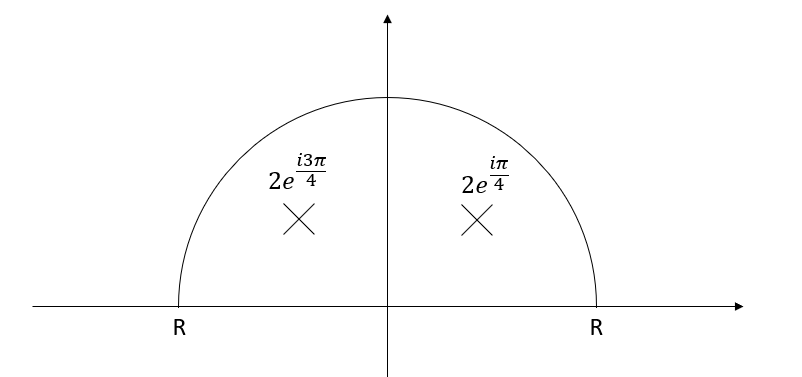
\includegraphics[scale=0.6]{Q4_diagram}
%\caption{Q4 diagram}
\end{figure}

There are 2 residue points inside the semicircle. Hence, by Cauchy Residue Theorem,
\[
\int_{-R}^R f(z)\ dz + \int_{\gamma_R} f(z)\ dz = 2\pi i(\Res_{z=2e^{\frac{i\pi}{4}}} f(z) + \Res_{z=2e^{\frac{i3\pi}{4}}} f(z))
\]
Now we want to find the residue at those 2 points.

\begin{align*}
\Res_{z=2e^{\frac{i\pi}{4}}} f(z) &= \lim_{z \to 2e^{\frac{i\pi}{4}}} (z-2e^{\frac{i\pi}{4}})f(z) \\
    &= \lim_{z \to 2e^{\frac{i\pi}{4}}} \frac{e^{iaz}}{4z^3} \\
    &= \frac{e^{-a\sqrt{2}}e^{ia\sqrt{2}}}{16\sqrt{2}(i-1)}
\end{align*}
\begin{align*}
\Res_{z=2e^{\frac{i3\pi}{4}}} f(z) &= \lim_{z \to 2e^{\frac{i3\pi}{4}}} (z-2e^{\frac{i\pi}{4}})f(z) \\
    &= \lim_{z \to 2e^{\frac{i3\pi}{4}}} \frac{e^{iaz}}{4z^3} \\
    &= \frac{e^{-a\sqrt{2}}e^{-ia\sqrt{2}}}{16\sqrt{2}(i+1)}
\end{align*}
Hence,
\[
\int_{-R}^R f(z)\ dz = 2\pi i\paren{\frac{e^{-a\sqrt{2}}e^{ia\sqrt{2}}}{16\sqrt{2}(i-1)} + \frac{e^{-a\sqrt{2}}e^{-ia\sqrt{2}}}{16\sqrt{2}(i+1)}} - \int_{\gamma_R} f(z)\ dz
\]
Hence,
\[
\int_{0}^R \frac{\cos (ax)}{x^4 + 16}\ dz = \frac{1}{2}\real \paren{2\pi i\paren{\frac{e^{-a\sqrt{2}}e^{ia\sqrt{2}}}{16\sqrt{2}(i-1)} + \frac{e^{-a\sqrt{2}}e^{-ia\sqrt{2}}}{16\sqrt{2}(i+1)}} - \int_{\gamma_R} f(z)\ dz}
\]
Now, we want to solve $\int_{\gamma_R} f(z)\ dz$:
\begin{align*}
\abs{\int_{\gamma_R} f(z)\ dz} \leq \pi R |f(z)| = \pi R \abs{\frac{e^{iaz}}{z^4 + 16}} \leq \pi R \frac{e^{-ay}}{|z^4| - 16} \leq \pi R \frac{1}{R^4 - 16}
\end{align*}
Which $\to 0$ as $R \to \infty$. Hence,
\begin{align*}
\int_{0}^\infty \frac{\cos (ax)}{x^4 + 16}\ dz &= \frac{1}{2}\real \paren{2\pi i\paren{\frac{e^{-a\sqrt{2}}e^{ia\sqrt{2}}}{16\sqrt{2}(i-1)} + \frac{e^{-a\sqrt{2}}e^{-ia\sqrt{2}}}{16\sqrt{2}(i+1)}}} \\
    &= -\pi \frac{e^{-a\sqrt{2}}}{16\sqrt{2}} \imm\paren{\frac{(-i-1)e^{ia\sqrt{2}}}{2} + \frac{(-i+1)e^{-ia\sqrt{2}}}{2}} \\
    &= -\frac{\pi}{2} \frac{e^{-a\sqrt{2}}}{16\sqrt{2}} \imm\paren{ (-i-1)e^{ia\sqrt{2}} + (-i+1)e^{-ia\sqrt{2}} } \\
    &= -\frac{\pi}{2} \frac{e^{-a\sqrt{2}}}{16\sqrt{2}} \paren{ -\cos(a\sqrt{2})  - \sin(a\sqrt{2}) - \cos(-a\sqrt{2}) + \sin(-a\sqrt{2})} \\
    &= -\frac{\pi}{2} \frac{e^{-a\sqrt{2}}}{16\sqrt{2}} \paren{ -2\cos(a\sqrt{2})  - 2\sin(a\sqrt{2})} \\
    &= \frac{\pi e^{-a\sqrt{2}}(\cos(a\sqrt{2} + \sin(a\sqrt{2})))}{16\sqrt{2}}
\end{align*}

Hence, for $a>0$,
\[
\int_{0}^\infty \frac{\cos (ax)}{x^4 + 16}\ dz = \frac{\pi e^{-a\sqrt{2}}(\cos(a\sqrt{2} + \sin(a\sqrt{2})))}{16\sqrt{2}}
\]
and for $a<0$,
\[
\int_{0}^\infty \frac{\cos (ax)}{x^4 + 16}\ dz = -\frac{\pi e^{-|a|\sqrt{2}}(\cos(|a|\sqrt{2} + \sin(|a|\sqrt{2})))}{16\sqrt{2}}
\]
\item
\begin{enumerate}
\item The only singular point is $z=0$.

\begin{align*}
\Res_{z=0} \frac{\exp(rz^n)}{z} &= \Res_{z=0} \frac{1}{z} (1 + rz^n + \frac{(rz^n)^2}{2} + \frac{(rz^n)^3}{3!} + \cdots) \\
    &= 1
\end{align*}

Then, by Cauchy residue theorem,
\[
\int_C \frac{\exp(rz^n)}{z}\ dz = 2\pi i
\]
\item Let the $C$ be the equation $e^{i\theta}$ for $0 \leq \theta \leq 2\pi$.
\begin{align*}
\int_C \frac{\exp(rz^n)}{z}\ dz &= \int_{0}^{2\pi} \frac{\exp(r(e^{i\theta})^n)}{e^{i\theta}} (ie^{i\theta})\ d\theta \\
    &= i \int_{0}^{2\pi} \exp(r(e^{i\theta})^n) \ d\theta \\
    &= 2\pi i
\end{align*}
\[
\therefore \int_{0}^{2\pi} \exp(r(e^{i\theta})^n) \ d\theta = 2\pi
\]
On the other hand,
\begin{align*}
\real \paren{\int_{0}^{2\pi} \exp(r(e^{i\theta})^n) \ d\theta} &= \real \paren{\int_{0}^{2\pi} \exp[\real(r(e^{i\theta})^n) + i\imm(r(e^{i\theta})^n)] \ d\theta} \\
    &= \real \paren{\int_{0}^{2\pi} \exp[r \cos(\theta n) + ir \sin(\theta n)] \ d\theta} \\
    &= \int_{0}^{2\pi} \real \paren{\exp[r \cos(\theta n) + ir \sin(\theta n)]} \ d\theta \\
    &= \int_{0}^{2\pi} \exp[r \cos(\theta n)] \real \paren{\exp[ir \sin(\theta n)]} \ d\theta \\
    &= \int_{0}^{2\pi} \exp(r \cos(\theta n)) \cos(r \sin(\theta n)) \ d\theta \\
\end{align*}
Hence,
\[\int_{0}^{2\pi} \exp(r \cos(\theta n)) \cos(r \sin(\theta n)) \ d\theta = \real(2\pi) = 2\pi\]
\end{enumerate}
\item
\begin{enumerate}
\item Consider the function $g(z) = (z - C)e^{i\frac{3\pi}{4}} + C$ (rotate $\frac{3\pi}{4}$ anti-clockwise about $C$.

\begin{figure}[h]
\centering
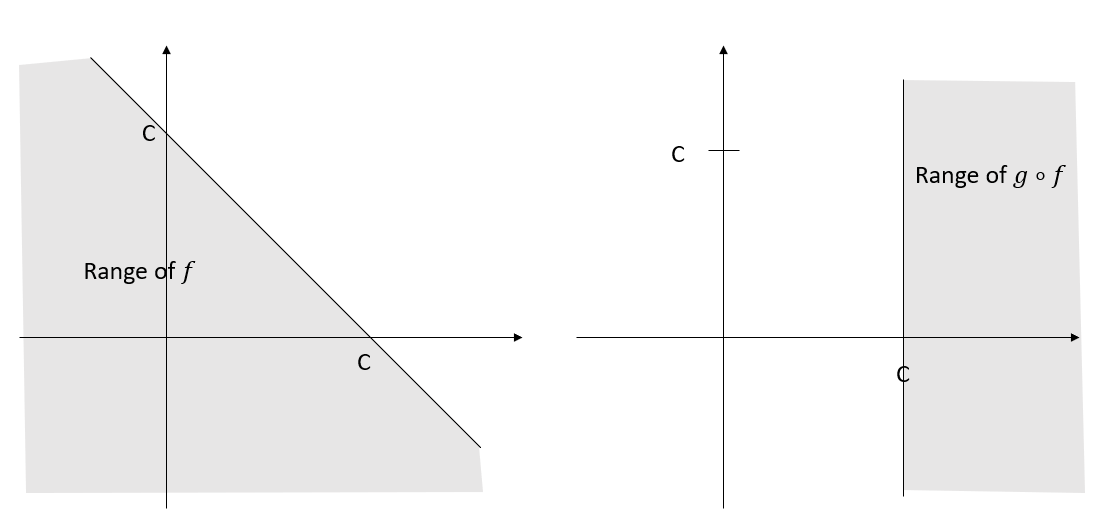
\includegraphics[scale=0.5]{Q6_diagram}
%\caption{Q6 diagram}
\end{figure}

Note that $\real(g(f(z)) \geq C$.

Then, consider $g_2(z) = \frac{1}{e^{z}}$.
\[|g_2(g(f(z)))| = \frac{1}{|e^{g(f(z))}|} \leq \frac{1}{C}\]

And since all of $f,g,g_2$ are analytic, and $g_2(g(f(z)))$ is bounded, hence, by Liouville's Theorem, $g_2(g(f(z)))$ is a constant, and hence, $g(f(z))$ is a constant, and hence, $f(z)$ is a constant.
\item Consider the function
\[
g(z) = \exp(f(z)-f(iz))
\]
This function is analytic. We want to show it is bounded.
\begin{align*}
|g(z)| &= |\exp(f(z)-f(iz))| \\
    &= \exp(\real(f(z)-f(iz))) \\
    &= \exp(u(x,y) - u(-y,x)) \\
    &\leq \exp(C)
\end{align*}
Hence, by Liouville's Theorem, $g(z) = \exp(f(z)-f(iz))$ is a constant. Hence, $f(z)-f(iz)=k$ for some constant $k \in \C$.

Substitute $z:=0$ into $f(z)-f(iz)=k$ to get $f(0)-f(0)=k$, hence, $k=0$. Hence,
\[f(z)=f(iz)\]
\end{enumerate}

\end{enumerate}

\end{document}
